\clearpage
\section{Recovered-RX clock counter and CDCE status: 15 November 2026}
Board PM12-K7-3A17A1B402212223 now retains SRAM build \texttt{ff2f746c}.
The original MCU and AUTO/PRIMARY clock configuration are unchanged. No persistent
programming or clock-profile changes were made. The SPI clock-loss finding remains open.

\subsection{Method and status register}
The independent counter domain uses GTX recovered RXOUTCLK before its RX MMCM
(RXOUTCLKSEL=2), nominally 60.11805 MHz from the Kasli serial stream.
Three free-running registered-Gray counters track CDCE U2/MCLK1, CDCE U3 divided
by two, and SYS. A window spans 384 reference cycles, approximately 6.387 microseconds.
A 2048-record circular buffer survives SYS reset and freezes on a sticky asynchronous
SYS-loss trigger. Full valid windows alone enter quantitative statistics.

TI SCAS862G Table 48 defines CDCE R8 payload bit 6 as PLLLOCKPIN and bits 27:25
as the selected input (1 PRIMARY, 2 SECONDARY, 4 AUX). The UART wire word includes
a low address nibble. Every before/after snapshot in all three trials was
\texttt{20009D38}: PRIMARY, PLL lock pin high. These fields report current state;
they are not documented sticky clock-loss or switching history. A short event can
occur between UART samples. Datasheet: \url{https://www.ti.com/lit/ds/symlink/cdce62005.pdf}.

\subsection{Measured results}
\begin{center}\begin{tabular}{lrrrrl}\toprule
Trial & Valid windows & MCLK & U3/2 & SYS & SYS trigger\\\midrule
Idle & 2047 & 256 & 640 & 256 & No\\
SPI read 0 & 1633 & 256--257 & 640--641 & 255--257 & Yes\\
SPI read 1 & 1616 & 256--257 & 639--641 & 256--257 & Yes\\\bottomrule
\end{tabular}\end{center}
Expected counts are 256/640/256, corresponding to 40.0787/100.19675/40.0787 MHz.
Both SPI signatures were correct. Deviations near SPI never exceeded one count:
endpoint CDC quantization and phase ambiguity prevent attributing these to an
extra physical pulse. The final partial reset-trigger record is excluded.
R8 provides no sampled evidence of an AUX switch; transient switching remains possible.

\begin{center}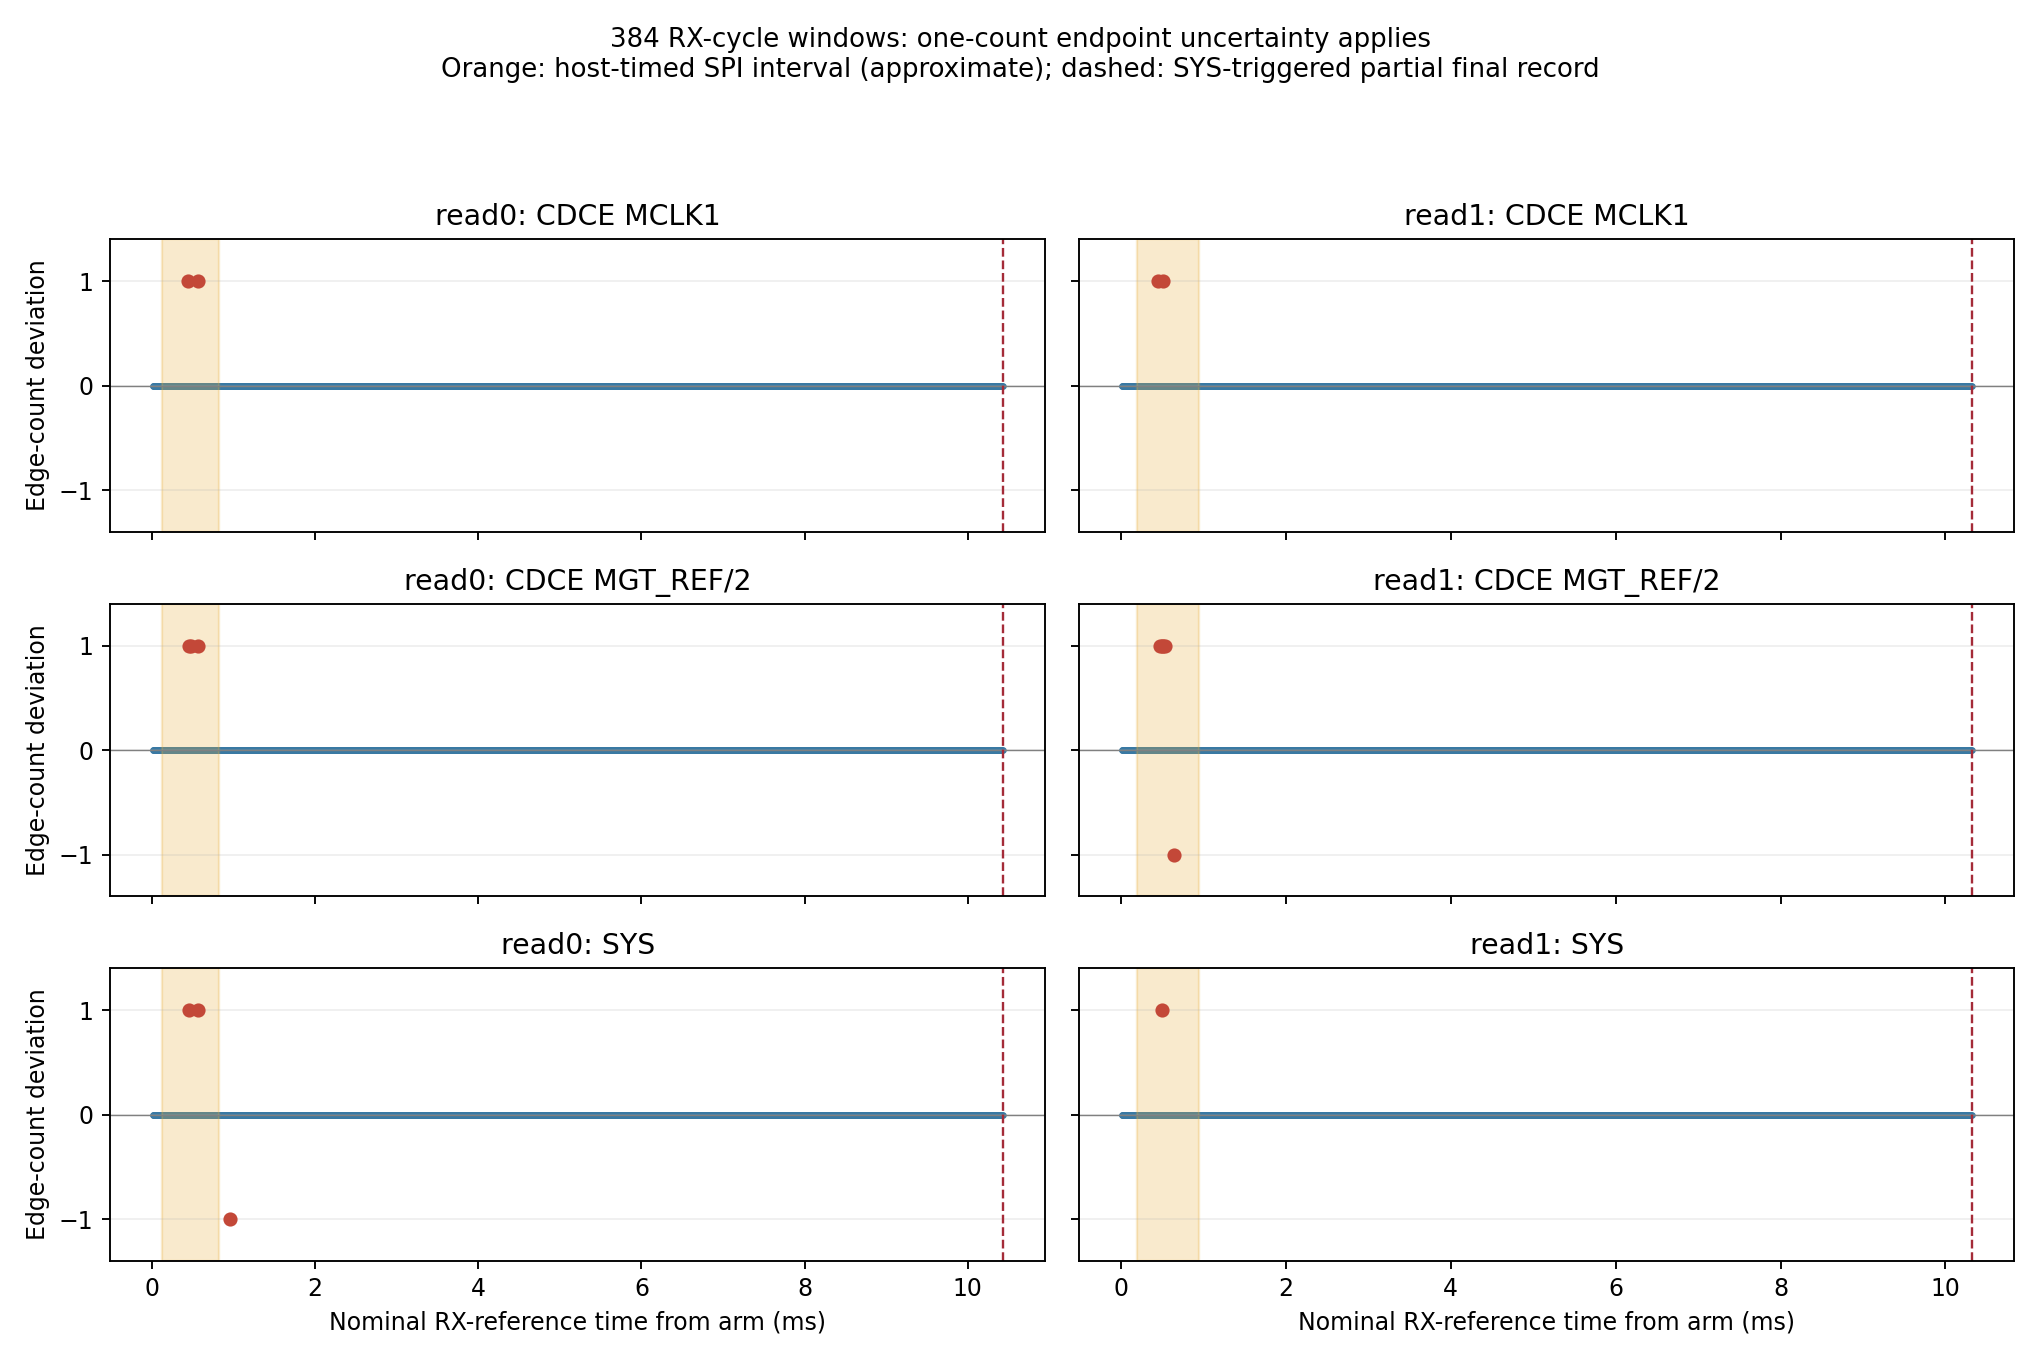
\includegraphics[width=\linewidth]{rx-clock-counter.png}\end{center}
Orange regions show approximate host SPI-call bounds. Red markers show SYS-loss
capture. The recovered reference depends on local GTX reference/CDR/reset circuitry:
it is not fully independent. Common stops, analog runt pulses and phase jumps can
escape this counter. No analog clock-integrity clearance is claimed.

\subsection{Qualification and retained state}
Simulation passed ratios, wrap, dropped-edge detection, invalid-reference marking,
reset capture, frozen retention and rearm. Dell implementation: WNS 0.016 ns,
WHS 0.063 ns; three Gray bus-skew maxima 0.528/0.497/0.889 ns, all below 5 ns.
Inherited clock-alias warnings remain. V1 used a misaligned RAM base and was
rejected before programming; tested V2 uses word address \texttt{a000}.
Final fresh reload passed power/frontend checks, ADT identity C3 and physical
ADC bank A on all 12 channels. Kasli outputs remain driven; leases released.

Raw buffers, scripts, exact V2 build and qualification receipts are archived in the
repository system diagnostics, under the dated recovered-RX counter evidence.
Original MCU remains unchanged.
